%%%%%%%%%%%%
%% Please rename this main.tex file and the output PDF to
%% [lastname_firstname_graduationyear]
%% before submission.
%%%%%%%%%%%%

\documentclass[12pt]{caltech_thesis}
\usepackage[hyphens]{url}
%\usepackage{lipsum} %dummy content
\usepackage{graphicx}

%\usepackage{todonotes}

\usepackage{hyperref}


%% Tentative: newtx for better-looking Times
\usepackage[utf8]{inputenc}
\usepackage[T1]{fontenc}
%\usepackage{newtxtext,newtxmath}

Must use biblatex to produce the Published Contents and Contributions, per-chapter bibliography (if desired), etc.
\usepackage[
backend=biber,natbib,
% IMPORTANT: load a style suitable for your discipline
%    style=authoryear
]{biblatex}



% Name of your .bib file(s)
%\addbibresource{coryBIB.bib}
%\addbibresource{example.bib}
%\addbibresource{ownpubs.bib}

\begin{document}

% Do remember to remove the square bracket!
%\title{Development of Excitation Channel for KAGRA Photon Calibratior}
%\author{Yu-Kuang Chu}
%
%\degreeaward{Master of Science}                 % Degree to be awarded
%\university{National Taiwan Normal University}    % Institution name
%\address{Taipei, Taiwan}                     % Institution address
%\unilogo{NTNU.png}                                 % Institution logo
%\copyyear{2018}  % Year (of graduation) on diploma
%\defenddate{[Exact Date]}          % Date of defense
%
%\orcid{[Author ORCID]}

%% IMPORTANT: Select ONE of the rights statement below.
% \rightsstatement{All rights reserved\todo[size=\footnotesize]{Choose one from the choices in the source code!! And delete this \texttt{todo} when you're done that. :-)}}
% \rightsstatement{All rights reserved except where otherwise noted}
% \rightsstatement{Some rights reserved. This thesis is distributed under a [name license, e.g., ``Creative Commons Attribution-NonCommercial-ShareAlike License'']}

%%  If you'd like to remove the Caltech logo from your title page, simply remove the "[logo]" text from the maketitle command
\maketitle[logo]
%\maketitle

\begin{acknowledgements} 	 
  Thank everyone ~~~
\end{acknowledgements}

\begin{abstract}
   [This abstract must provide a succinct and informative condensation of your work. Candidates are welcome to prepare a lengthier abstract for inclusion in the dissertation, and provide a shorter one in the CaltechTHESIS record.]
\end{abstract}

%% Uncomment the `iknowhattodo' option to dismiss the instruction in the PDF.
%\begin{publishedcontent}%[iknowwhattodo]
%% List your publications and contributions here.
%\nocite{Cahn:etal:2015,Cahn:etal:2016}
%\end{publishedcontent}

\tableofcontents
\listoffigures
\listoftables
\printnomenclature
\mainmatter





\chapter{Introduction} 

When you got a new camera, you probably will take a lot of testing photos before you start to use it seriously. Similarly, we would like to test our gravitational wave detector before we use it to see the Universe.

Hardware injection test is a process to verify the performance of interferometer by sending sample signals into interferometer. Ideally, we should prepare some real gravitational waves as test signals. But it is practically hard to generate large enough artificial gravitational waves that are detectable by current technology. 

Therefore, instead of generating gravitational waves, people mimic the effect of celestial gravitational waves by displacing the mirror according to the simulated gravitational waveforms, changing arm length correspondingly, , comparing the optical readout in the main interferometer, thereby checking the response of their interferometer. 

Among different ways to push those Test Mass Mirrors in the main interferometer, radiation pressure of external laser beams have been used because its simplicity and stability. A dedicated auxiliary laser system called Photon Calibrator(PCal) has been developed for this purpose. 

In this dissertation, I will briefly explain what is photon calibrator and how it works for calibration and hardware injection purposes. Then, I will discuss the noise problem from current signal generating system that is used to control PCal Laser intensity. Finally, a possible solution, Analog De-Whitening Filter, has been manufactured and tested with Photon Calibrator in Kamioka Gravitational Wave Detector (KAGRA). 
 

\section{Introduction to Gravitational Wave}
\subsection{What is gravitational wave}

In the General Theory of Relativity proposed by Albert Einstein in 1915, phenomena caused by gravity can be interpreted as results of curved spacetime. This is one of his important works after his `Happiest Thought', which recorded in his unpublished article ``Fundamental Ideas and Methods of the Theory of Relativity, Presented in Their Development"\cite{Einstein:happy}. Among different ways to curve our spacetime, which can be described by corresponding metric tensor fields, there exist wavelike solutions describing ripples of spacetime known as gravitational waves.

However, the physical reality of gravitational wave was not so clear to everyone in the early days, even to Einstein himself~\cite{Einstein:prl, Einstein:ongw}. The main problem is that there exist some gauge degree of freedom in the theory due to the arbitrariness of coordinate choices. We have to know whether the gravitational waves we found are just gauge waves (vibration of coordinate) or the wave can have some observable consequences. 

One of the most important observational evidence implying the existence of real gravitational waves is the Hulse-Taylor pulsar~\cite{HulseTaylor:discovery}. Taylor demonstrated that the change of pulsar rotation speed can be explained by emission of gravitational wave~\cite{HulseTaylor:gr, HulseTaylor:gr2}.  

% in 2015 September 14th
Finally, on September 14th, 2015, the first direct detection of gravitational wave signal~\cite{gw:150914_det} is done by Laser Interferometer Gravitational-Wave Observatory(LIGO) detectors in the United States.

\subsection{How to describe gravitational wave}

In Einstein's General Relativity, gravitational effects are realized by geometry of spacetime. According to a great mathematician Bernhard Riemann, we can describe the geometry of certain space by telling the ``distance" between nearby points in the space. Practically, the information of distance between nearby spacetime points form a tensor called metric, which means the measure of distance. By choosing a coordinate system, one can write down those corresponding components of metric tensor $g$.
\begin{equation}
    g_{\mu\nu}=
\left(
\begin{array}{cccc}
  g_{00} & g_{01} & g_{02} & g_{03} \\
  g_{10} & g_{11} & g_{12} & g_{13} \\
  g_{20} & g_{21} & g_{22} & g_{23} \\
  g_{30} & g_{31} & g_{32} & g_{33}
\end{array}
\right)  
\end{equation}
 Now, we can calculate spacetime distance $ds$ between two nearby points by their coordinate separation:

\begin{equation}
    ds^2 = g_{\mu\nu} dx^{\mu} dx^{\nu}
\end{equation}




\begin{figure}[hbt!]
\centering
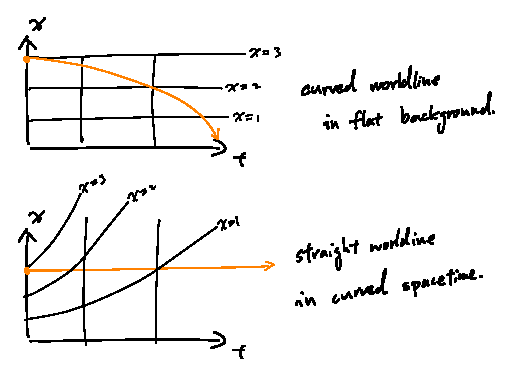
\includegraphics[width=0.8\textwidth]{figure/gr/curvedxt.eps}
\caption{Newtonian versus Einstein's point of view. }\label{fig:grxt}
\index{figures}
\end{figure}


Through the interaction between matter and spacetime, matter can curve our Universe. The whole story can be resolved by solving Einstein equation,
\begin{equation}
\label{eq:einsteineq}
    R_{\mu\nu}-\frac{1}{2}g_{\mu\nu}R = \frac{8 \pi G}{c^4} T_{\mu\nu}
\end{equation}
which is a non-linear differential equation of metric tensor field $g_{\mu\nu}(x^{\alpha})$ since the Ricci tensor $R_{\mu\nu}$ contains metric tensor and its differential.

It's similar to the case in Electrodynamics, in which we can have electromagnetic waves solutions by solving Maxwell equations in vacuum, that we can have gravitation wave solutions by solving vacuum Einstein equation. The situation will become even clear if we linearize the Einstein equation and choose coordinate or gauge properly.

%Gravitational phenomenon can be thought as the interaction between matter(Energy-Stress Tensor field) and the spacetime(Metric Tensor filed). This is similar to the case in Electrodynamics, in which the interaction between electrical charges and electrical/magnetic fields give us EM phenomenon. The mathematical formulae that govern EM phenomenon are Maxwell equations. 
% Given the the spacetime filled with metric tensor field which tell us the shape or geometry of our universe. 
 
 Let's start from 





\begin{equation}
    \Box \bar{h}_{\mu\nu} = - \frac{16\pi G}{c^4}T_{\mu\nu}
\end{equation}


%When it comes to gravitational wave, there is a very convenient gauge(coordinate) constrain called Traceless and Transverse gauge. 


the corresponding coordinates are attached to a set of free falling objects. 
for perturbation of wave like part metic over Schwarzschild background which represent Earth’s gravity.


Refer to \cite{maggiore:gw1}



How to generate gravitational wave
The source of electromagnetic wave is time-dependent electrical charge distribution.  Similarly, the source of gravitational wave is time-dependent mass(energy) distribution. Strictly speaking, the lowest order of mass multi-pole which can generate real gravitational waves is mass quadruple because we don’t have negative mass, while the electromagnet wave can be generate though time-dependent electrical dipole moment. The gravitational wave strain generated by mass quadruple can be approximately described by famous quadrupole formula:
(quadrupole formula)
Practically, PN NR....
According to our current understand of universe, there are several kinds of astrophysical gravitational wave sources, whose h(t) amplitude is large enough to be detected by current ground based laser interferometer, like advanced-LIGO, advanced-Virgo or KAGRA. 
Compact Binary Coalescence 
BNS BBH
\subsection{How to detect Gravitational wave}
The interaction of detector and gravitational wave can have different interpretation due to different coordinate choice\cite{ifo:gauge}. It is quiet similar to that the magnetic force in one observational frame may be electric force in the other frame. However, practically, I would like to use the …….., which described in next section.


\section{Detection of Gravitation wave}

Interaction of GW wave when $\lambda_gw$ L of detector
Limit of Michelson IFO
IFO with dual-recycling and Fabry-Perot  arms.
 Complex response
WE NEED Calibration Calibration Calibration



\section{Calibration and Reconstruction}

Calibration is always the fist step before we measure something by some device.
For example, to measure the weight of an apple, you should calibrate your scale by putting a “standard kilogram” on it. Then, you can either adjust the scale readout to be 1kg, or record the difference showed in scale readout, which may be used to reconstruct real weight of the apple. However, the spring constant of springs inside the scale could fluctuate due to temperature changes. To accurately measure the weight of the apple, we have to measure the calibration factor (scale readout when we put the standard mass on it.) when we measure the weight of apple, if possible, simultaneously.

Due to the complexity of practical interferometer, the response of interferometer itself to external gravitational source is not only sophisticated but also time-dependent. In reality, we “inject several calibration lines”, which means we displace the End-Test-Mirror by several known frequency and amplitude sine waves. Then, we try to see these standard signals in the readout of interferometer, thereby solving the response of interferometer.

\subsection{Transfer function of Laser Interferometer with Fabry-Perot Cavity}


\subsection{Tracking Time-dependent Response by Calibration lines}



\section{Photon Calibrator (Pcal)}
\subsection{Principle of Photon Calibrator}
Photon calibrator is an additional laser with high precision intensity modulator. It is installed in front of End-Test-Mass Mirror(ETM) and can push the ETM by radiation force due to its own Laser beam as depicted in Fig.(XX). To generate any artificial h(t) by Pcal, we have to translate desired h(t) into corresponding force F(t) exerting on ETM. This can be done by using equation of motion of the ETM suspend by its suspension system. Then, we control the Pcal Laser output intensity P(t) such that the radiation force exerted on ETM is F(t) we calculated before. 

The radiation force caused by a continuous laser beam can be calculated by its momentum transfer per unit time.

\begin{equation}
    \mathbf{F} = \frac{\Delta \mathbf{p}}{\Delta t}
\end{equation}
For our purpose, the laser beam will be almost reflected from ETM. Therefore, the momentum transfer to ETM per unit time should be almost equal to twice of longitudinal momentum flux carried by PCal laser beam.

\begin{equation}
\label{eq:f2cos}
    \mathbf{F}_\text{on ETM} = \frac{\Delta \mathbf{p}_\text{ETM}}{\Delta t}
    = 2 \cos(\theta) \frac{\Delta p_\text{Laser} }{\Delta t}
\end{equation}
where $\theta$ is the angle of incident.

Furthermore, one can express the momentum flux of light in terms of its intensity through Eq.(\ref{eq:epc}), which can be derived from either classical point of view with its Poynting vector or Quantum Mechanical approaches that we adopt here by dealing with photons. 

\begin{align}
   E_{\gamma} &= \hbar \omega \\
   p_{\gamma} &= \hbar k \\
              &= \frac{k}{\omega} ~ E_{\gamma} = \frac{1}{c}E_{\gamma}
\end{align}

\begin{align}
\label{eq:epc}
   \underbrace{\frac{\Delta p_{\text{photons}}}{\Delta t}}_{\text{momentum flux due to }\atop \text{photons in a continuous laser beam}}
   &= \frac{1}{c}
   \underbrace{ \frac{\Delta E_{\text{photons}}}{\Delta t} }_{\text{Intensity of laser beam}\atop \text{defined as } P}
   = \frac{P}{c} 
\end{align}

%\begin{align}
%    E_{\gamma} &= \hbar \omega \\
%    p_{\gamma} &= \hbar k \\
%               &= \frac{k}{\omega} ~ E_{\gamma} = \frac{1}{c}E_{\gamma}   \\
%    \frac{\Delta p_{\text{photons}}}{\Delta t}
%    &= \frac{1}{c} \frac{\Delta E_{\text{photons}}}{\Delta t} 
%    = \frac{P}{c} 
%\end{align}
Combining Eq.(\ref{eq:f2cos}) and Eq.(\ref{eq:epc}), the force that PCcal can give ETM is:

\begin{equation}
\label{eq:pcalforce}
    F_\text{PCal}(t) = \frac{ 2 \cos(\theta) }{c} P(t) 
\end{equation}


On the other hand, the equation of motion of suspend ETM can be modeled as:

\begin{equation}
\label{eq:etmeom}
    \ddot{x}(t) + b \dot{x}(t) + \omega_0^2 x(t) = \frac{F(t)}{M} 
%    F_\text{PCal}(t) = \frac{ 2 \cos(\theta) }{c} P(t) 
\end{equation}

%The solution to Eq.(\ref{eq:etmeom}) can be wrote as the combination of homogeneous part and particular solution:
%
%\begin{equation}
%%\label{eq:etmeom}
%    x(t)=x_h(t)+x_p(t)
%\end{equation}


The impulse response is

\begin{equation}
%\label{eq:etmeom}
    x(t)=\frac{b}{\omega_1}e^{-\frac{b}{2}(t-t_0)}\sin[\omega_1 (t-t_0)]
\end{equation}


And the transfer function is

\begin{equation}
\label{eq:etmtf}
   x(\omega)=\frac{-1}{\omega^2 - \omega_0^2 + i \omega b}F(\omega)
\end{equation}

As long as $\omega^2 \gg \omega_0^2$ and $\omega \gg b$, Eq.(\ref{eq:etmtf}) can be approximated as

\begin{equation}
%\label{eq:etmtf}
   x(\omega)=\frac{-1}{\omega^2}F(\omega)
\end{equation}

By substituting the Fourier transformed Eq.({\ref{eq:pcalforce}}) into it, we can get the expression of x(f) introduced by P(f)
\begin{equation}
\label{eq:pcaldisp}
    x(\omega) = \frac{-1}{M \omega} \frac{2  P(f) \cos(\theta)}{c} 
\end{equation}



\subsection{Evolution of Photon Calibrator}

Original Pcal is proposed by Glasgow group \cite{pcal:clubley2001}. They use single laser beam hitting on the center of ETM and successfully see these sin waves in the the readout of their interferometer. Later on, GEO...

 is that it may introduce drumhead mode vibration of ETM surface (just like the vibration mode you see when you hit the center of a drum), which introduce unwanted h(t) effectively. This problem is solved by LIGO group\cite{pcal:karki2016}, who separate the Pcal laser beam into two beams, hitting on the nodal point of drumhead mode on the ETM surface\cite{pcal:Daveloza2012}.  


In order to excite same amplitude h(t) in higher frequency regime, we have to give much larger F(t) since the relationship between x(t) and F(t) in an pendulum ……………….



\subsection{Why do we need Photon Calibrator}
\subsection{Tracking Time-dependent Response by Calibration lines}


\chapter{Hardware Injection through Photon Calibrator}
\section{Principle}



 
 As I described in Sec.\ref{sec:pcalth}, we can generate desired ETM displacement $x(t)$ by changing PCal laser intensity $P(t)$. One can calculate corresponding $P(t)$ by performing inverse Fourier transform to Eq.(\ref{eq:pcaldisp}).
 
\begin{align}
    \int_{-\infty}^{-\infty} x(\omega) e^{i \omega t} ~\mathrm{d} \omega &= 
     \frac{-2   \cos(\theta)}{Mc} 
     \int_{-\infty}^{-\infty}\frac{P(\omega)}{\omega^2} e^{i \omega t} ~\mathrm{d} \omega \\
\label{eq:pcaldispt}
    \frac{Mc}{-2 \cos(\theta)} \int_{-\infty}^{-\infty}
     x(\omega) \omega^2 e^{i \omega t} ~\mathrm{d} \omega 
&= P(t) 
\end{align}

where
\begin{align*}
%\label{eq:pcaleq}
   \text{Mass of ETM} \qquad  M &= 23 ~\mathrm{kg} \\
   \text{Arm Length} \qquad   L &= 3 ~\mathrm{km}  \\
   \text{Angle of Incident} \qquad   \theta &= 0.72 ~\mathrm{deg}  \\
   \text{Speed of Light} \qquad   c &= 2.998\times10^8 ~\mathrm{m/s} \\
\end{align*}
Also, if we have complete suspension model of ETM, we can substitute the $\omega^2$ factor in Eq.(\ref{eq:pcaldispt}) by the full displacement-to-force transfer function.


\pagebreak
\section{Experimental Setup}

Once we got the necessary P(t) from the desired x(t) through Eq.(\ref{eq:pcaldispt}), we can start to modulate our PCal laser intensity according to that P(t). The way how we control our PCal laser intensity is explained in Fig.~(\ref{fig:injsigpath}).


\begin{figure}[hbt!]
\centering
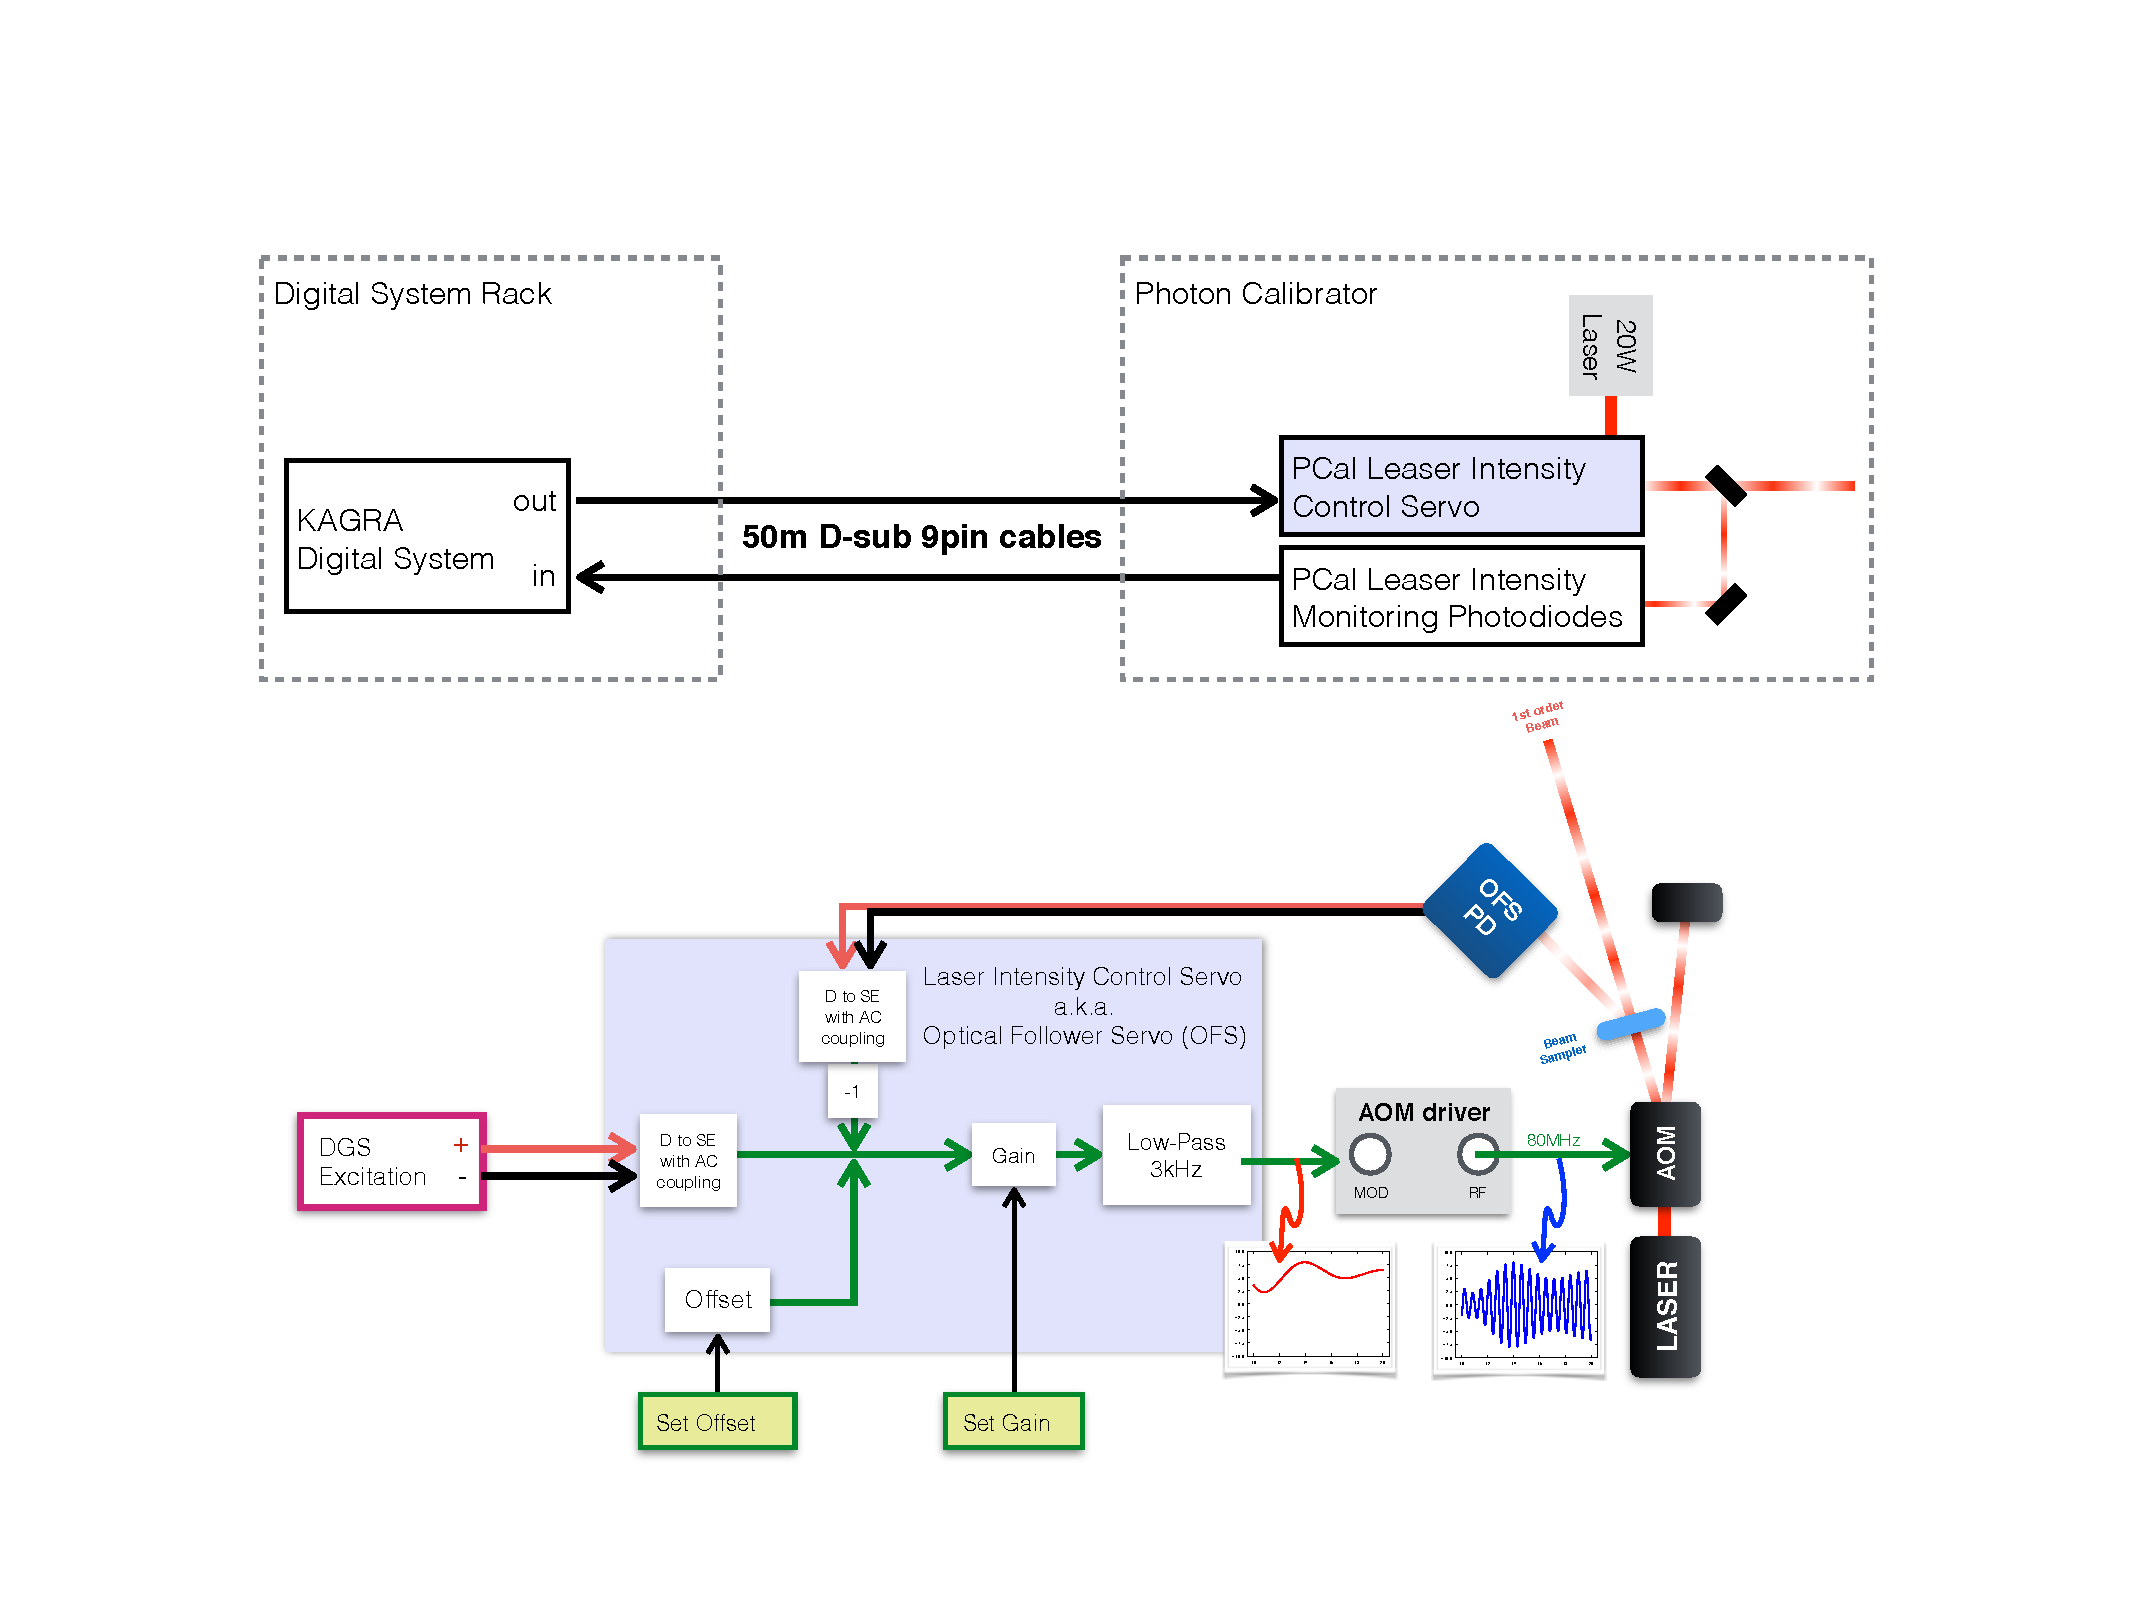
\includegraphics[width=1\textwidth]{figure/injsigpath}
\caption[Controlling PCal with Digital Control System]{Controlling PCal with Digital Control System. The PCal laser beam that will be sent to ETM is the first order diffracted beam of a 20W input laser form an acousto-optic modulator(AOM). Its intensity is controlled by the control signal from our KAGRA Digital System. An analog feedback control loop called Optical Follower Servo(OFS) has been implemented to reduce non-linear response of AOM and laser intensity noise of 20W input laser.  }
\label{fig:injsigpath}
\index{figures}
\end{figure}


%
%Validate IFO by Pcal (Hardware Injection Test)
%As I mentioned in last chapter, the practical response of IFO is very complex. To prevent some unexpected problem including no-linear response of IFO and……  
%The best way is to provide some test source of expected GW signal.
%
%However, it is almost impossible to prepare, for example, a binary blackhole system in laboratory. Instead, we will generated some test signal by pushing the ETM with Pcal. This procedure is called “Hardware Injection Test”
%
%
%Motivation
%To under whether we can successfully reconstruct the h(t) from our interferometer, the best way is to prepare an artificial signal, sending it to interferometer, reconstructing it, finally, comparing it with original one. However it is quite difficult to generate human made gravitational wave that can be detected by current gravitational wave detector.
%
%Requirement
%
%Low Frequency
%around 100Hz  the nose should below the IFO sensitivity
%(absolute timing < ?us ns )
%
%High Frequency
%above 1kHz    the transfer function should as flat as possible


%\subsubsection{Amplitude of Injection Signal}

%\begin{equation}
%\label{eq:pcaleq}
%    \Delta L (f) (\mathrm{m} / \mathrm{Hz}) = \frac{2 \Delta P \cos(\theta)}{c} \frac{1}{M (2 \pi f )^2}
%\end{equation}
%
%\begin{align}
%%\label{eq:pcaleq}
%    \frac{F(t)}{M}=\frac{1}{M} \frac{2 P(t) \cos(\theta)}{c} &= \ddot{x}(t)
%\end{align}
%
%For $x=x_0 \sin(\omega t)$,
%\begin{align}
%%\label{eq:pcaleq}
%    \frac{1}{M} \frac{2 P_0 \cos(\theta)}{c} \sin(\omega t) &=  -\omega^2 x_0 \sin(\omega t)
%\end{align}
%
%Thus,
%\begin{align}
%%\label{eq:pcaleq}
%    P_0 &= -\omega^2 \frac{M c}{2 \cos(\theta)} x_0 = -\omega^2 \frac{M c}{2 \cos(\theta)} L h_0
%\end{align}







%\begin{align*}
%%\label{eq:pcaleq}
%    P_0 ~(\mathrm{Watts}) \times \frac{Gain_{\text{~Power to OFSPD}}}{2} &= 
%     \underbrace{V_{\text{OFSPD}}}_{\text{Same as V$_{\text{Injection}}$}}~ (\mathrm{Volts}) \\
%\end{align*}
%Therefore, the overall gain should be set in injection channel, which is in Volt unit, is
%\begin{align}
%%\label{eq:pcaleq}
%    \omega^2 \frac{M c}{2 \cos(\theta)} L \times \frac{Gain_{\text{~Power to OFSPD}} }{2}
%\end{align}


\chapter{Development of Injection Channel}

\section{Requirement of Injection Channel}
\subsection{Noise Requirement}

\begin{figure}[hbt!]
\centering
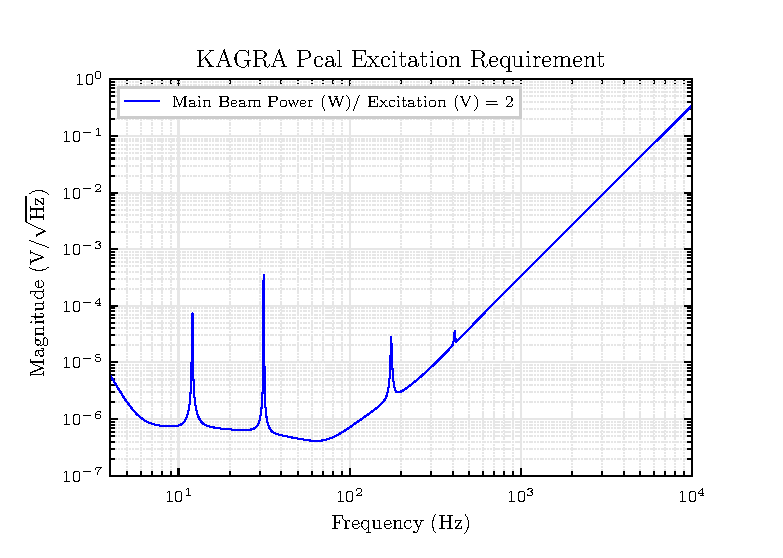
\includegraphics[width=.9\textwidth]{figure/DAC_requirement.eps}
\caption{Injection Channel Noise Requirement}\label{fig:DAC_noise_requirement}
\index{figures}
\end{figure}

\begin{align}
%\label{eq:}
   \Delta L(f) &< \frac{1}{10} \times (\text{KAGRA length sensitivity})\\
   \Delta L(f) =\frac{2 \Delta P(f) \cos(\theta)}{c} \frac{1}{M(2 \pi f)^2} &< \frac{1}{10} \Delta h(f) L
\end{align}








\section{Noise Source of Excitation channel}
\subsection{Quantization Noise of DAC}


The origin of quantization error is coming from the difference between desired analog output and quantized Digital to Analog Converter(DAC) output value. Roughly speaking, it shows like white noise spreading from DC to Nyquist frequency i.e. $Fs/2$.
The Root Mean Square value of quantization noise has the order of voltage difference corresponding to last digit or Least Significant Bit(LSB). In time domain, we can calculate standard deviation.
\begin{align}
%\label{eq:}
   \sigma_x = \sqrt{\frac{1}{12}} \delta x_{LSB}
\end{align}

For a 16-bit 64kHz DAC with output range between $\pm 10$Volts, 
\begin{align}
%\label{eq:}
    \sigma_x &= \sqrt{\frac{1}{12}} \delta x_{LSB} \\
             &= \sqrt{\frac{1}{12}} \frac{(+10)-(-10) \mathrm{Volts}}{2^{16}} \\
             &= 8.81 \times 10^{-5} \;\mathrm{Volts}
\end{align}

In frequency Domain, the quantization noise is distributed from DC to 32768Hz; therefore, we have ASD
\begin{align}
%\label{eq:}
    ASD &= \sqrt{PSD} \\
        &= \sqrt{ \frac{\sigma_x^2}{32768} } \\
        &= 8.81 \times 10^{-5} \sqrt{\frac{1}{32768}} \\
        &= 4.87 \times 10^{-7} \;\mathrm{Volts}/\sqrt{\mathrm{Hz}} 
\end{align}





\section{Noise Reduction through de-whitening filter}
Problem of 16kHz excitation channel 
Implementation of 64kHz Excitation channel in KAGRA digital system

Principle of Analog filter
Design of De-Whitening filter
Performance test
Transfer function measurement 
Noise requirement
Create Inverse De-Whitening filter






\chapter{Validation of Injection Channel}
Noise measurement
around 100Hz  the nose should below the IFO sensitivity
Transfer Function measurement
“above 1kHz” performance
time delay of excitation channel
(absolute timing measurement?)
Distortion of Scientific Signal
BBH
BNS post merger




\cite{a:b}


%
\bibliographystyle{unsrt}
\bibliography{cory}

%\printbibliography[heading=bibintoc]

%\appendix
%\printindex
%\theendnotes

%% Pocket materials at the VERY END of thesis
%\pocketmaterial
%\extrachapter{Pocket Material: Map of Case Study Solar Systems} 


\end{document}
